\documentclass[letterpaper,12pt]{article}
\usepackage[margin=.65in,top=.72in,bottom=.62in,headheight=16pt,headsep=15pt,footskip=19pt]{geometry}
\usepackage[T1]{fontenc}
\usepackage{lmodern,tikz,fancyhdr}\pdfmapfile{+lm.map}
\usetikzlibrary{arrows.meta,shapes.geometric}
\pagestyle{fancy}\fancyhf{}\renewcommand{\headrulewidth}{0pt}\renewcommand{\footrulewidth}{0pt}
\setlength{\parindent}{0pt}\setlength{\parskip}{0pt}
\fancyhead[L]{\small Week 42 / Fair results from a bag / Grades 4--5}
\fancyfoot[L]{\footnotesize Bellingham Math Circle / Week 42 / W42-grades-4-5-v2}\fancyfoot[R]{\footnotesize\thepage}
\begin{document}
\noindent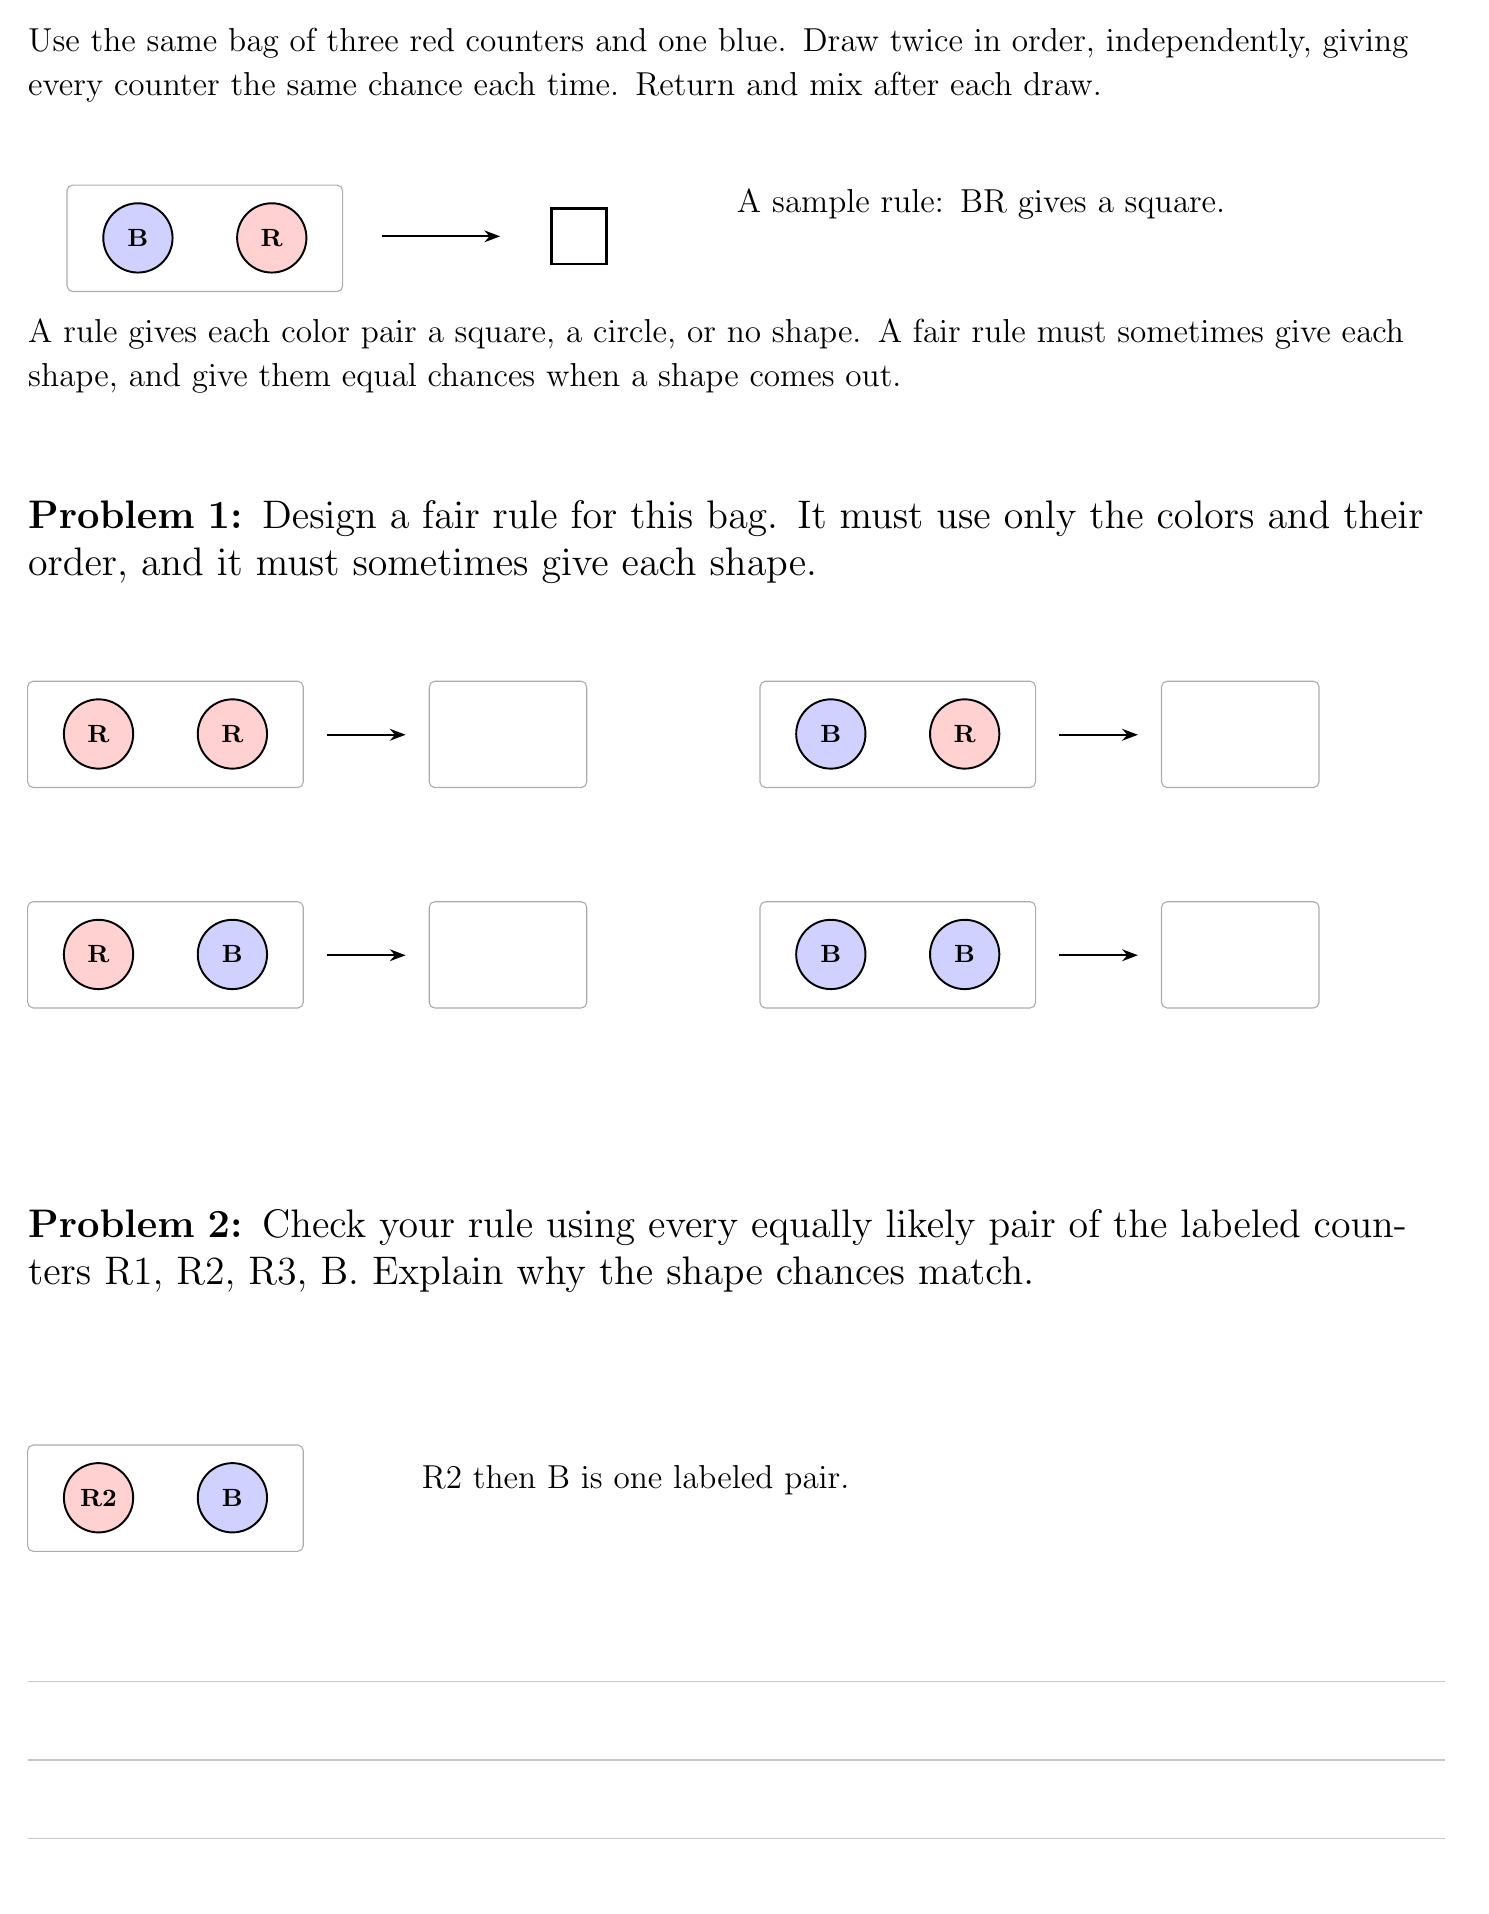
\begin{tikzpicture}[x=1cm,y=1cm]\path[use as bounding box] (0,0) rectangle (18.2,-23.6);
\node[anchor=north west,text width=18cm,inner sep=0pt,font=\fontsize{13}{16}\selectfont] at (0,0) {Use the same bag of three red counters and one blue. Draw twice in order, independently, giving every counter the same chance each time. Return and mix after each draw.};
\draw[gray!65,rounded corners=2pt] (0.5,-2) rectangle (4.0,-3.35);
\draw[fill=blue!18,line width=.7pt] (1.4,-2.67) circle (0.44);
\node[font=\bfseries\small] at (1.4,-2.67) {B};
\draw[fill=red!18,line width=.7pt] (3.1,-2.67) circle (0.44);
\node[font=\bfseries\small] at (3.1,-2.67) {R};
\draw[-{Stealth[length=2mm]},line width=.8pt] (4.5,-2.65) -- (6,-2.65) node[midway,above,font=\small] {};
\draw[line width=1pt] (6.65,-3.0) rectangle (7.35,-2.3);
\node[anchor=north west,text width=8.5cm,inner sep=0pt,font=\fontsize{12}{15}\selectfont] at (9,-2.05) {A sample rule: BR gives a square.};
\node[anchor=north west,text width=18cm,inner sep=0pt,font=\fontsize{13}{16}\selectfont] at (0,-3.7) {A rule gives each color pair a square, a circle, or no shape. A fair rule must sometimes give each shape, and give them equal chances when a shape comes out.};
\node[anchor=north west,text width=18cm,inner sep=0pt,font=\fontsize{14}{17}\selectfont] at (0,-6) {\textbf{Problem 1:} Design a fair rule for this bag. It must use only the colors and their order, and it must sometimes give each shape.};
\draw[gray!65,rounded corners=2pt] (0,-8.3) rectangle (3.5,-9.65);
\draw[fill=red!18,line width=.7pt] (0.9,-8.97) circle (0.44);
\node[font=\bfseries\small] at (0.9,-8.97) {R};
\draw[fill=red!18,line width=.7pt] (2.6,-8.97) circle (0.44);
\node[font=\bfseries\small] at (2.6,-8.97) {R};
\draw[-{Stealth[length=2mm]},line width=.8pt] (3.8,-8.98) -- (4.8,-8.98) node[midway,above,font=\small] {};
\draw[gray!65,rounded corners=2pt] (5.1,-8.3) rectangle (7.1,-9.65);
\draw[gray!65,rounded corners=2pt] (0,-11.100000000000001) rectangle (3.5,-12.450000000000001);
\draw[fill=red!18,line width=.7pt] (0.9,-11.770000000000001) circle (0.44);
\node[font=\bfseries\small] at (0.9,-11.770000000000001) {R};
\draw[fill=blue!18,line width=.7pt] (2.6,-11.770000000000001) circle (0.44);
\node[font=\bfseries\small] at (2.6,-11.770000000000001) {B};
\draw[-{Stealth[length=2mm]},line width=.8pt] (3.8,-11.780000000000001) -- (4.8,-11.780000000000001) node[midway,above,font=\small] {};
\draw[gray!65,rounded corners=2pt] (5.1,-11.100000000000001) rectangle (7.1,-12.450000000000001);
\draw[gray!65,rounded corners=2pt] (9.3,-8.3) rectangle (12.8,-9.65);
\draw[fill=blue!18,line width=.7pt] (10.200000000000001,-8.97) circle (0.44);
\node[font=\bfseries\small] at (10.200000000000001,-8.97) {B};
\draw[fill=red!18,line width=.7pt] (11.9,-8.97) circle (0.44);
\node[font=\bfseries\small] at (11.9,-8.97) {R};
\draw[-{Stealth[length=2mm]},line width=.8pt] (13.100000000000001,-8.98) -- (14.100000000000001,-8.98) node[midway,above,font=\small] {};
\draw[gray!65,rounded corners=2pt] (14.4,-8.3) rectangle (16.4,-9.65);
\draw[gray!65,rounded corners=2pt] (9.3,-11.100000000000001) rectangle (12.8,-12.450000000000001);
\draw[fill=blue!18,line width=.7pt] (10.200000000000001,-11.770000000000001) circle (0.44);
\node[font=\bfseries\small] at (10.200000000000001,-11.770000000000001) {B};
\draw[fill=blue!18,line width=.7pt] (11.9,-11.770000000000001) circle (0.44);
\node[font=\bfseries\small] at (11.9,-11.770000000000001) {B};
\draw[-{Stealth[length=2mm]},line width=.8pt] (13.100000000000001,-11.780000000000001) -- (14.100000000000001,-11.780000000000001) node[midway,above,font=\small] {};
\draw[gray!65,rounded corners=2pt] (14.4,-11.100000000000001) rectangle (16.4,-12.450000000000001);
\node[anchor=north west,text width=18cm,inner sep=0pt,font=\fontsize{14}{17}\selectfont] at (0,-15) {\textbf{Problem 2:} Check your rule using every equally likely pair of the labeled counters R1, R2, R3, B. Explain why the shape chances match.};
\draw[gray!65,rounded corners=2pt] (0,-18) rectangle (3.5,-19.35);
\draw[fill=red!18,line width=.7pt] (0.9,-18.67) circle (0.44);
\node[font=\bfseries\small] at (0.9,-18.67) {R2};
\draw[fill=blue!18,line width=.7pt] (2.6,-18.67) circle (0.44);
\node[font=\bfseries\small] at (2.6,-18.67) {B};
\node[anchor=north west,text width=12cm,inner sep=0pt,font=\fontsize{12}{15}\selectfont] at (5,-18.25) {R2 then B is one labeled pair.};
\draw[gray!45] (0,-21) -- (18,-21);
\draw[gray!45] (0,-22) -- (18,-22);
\draw[gray!45] (0,-23) -- (18,-23);
\end{tikzpicture}
\newpage
\noindent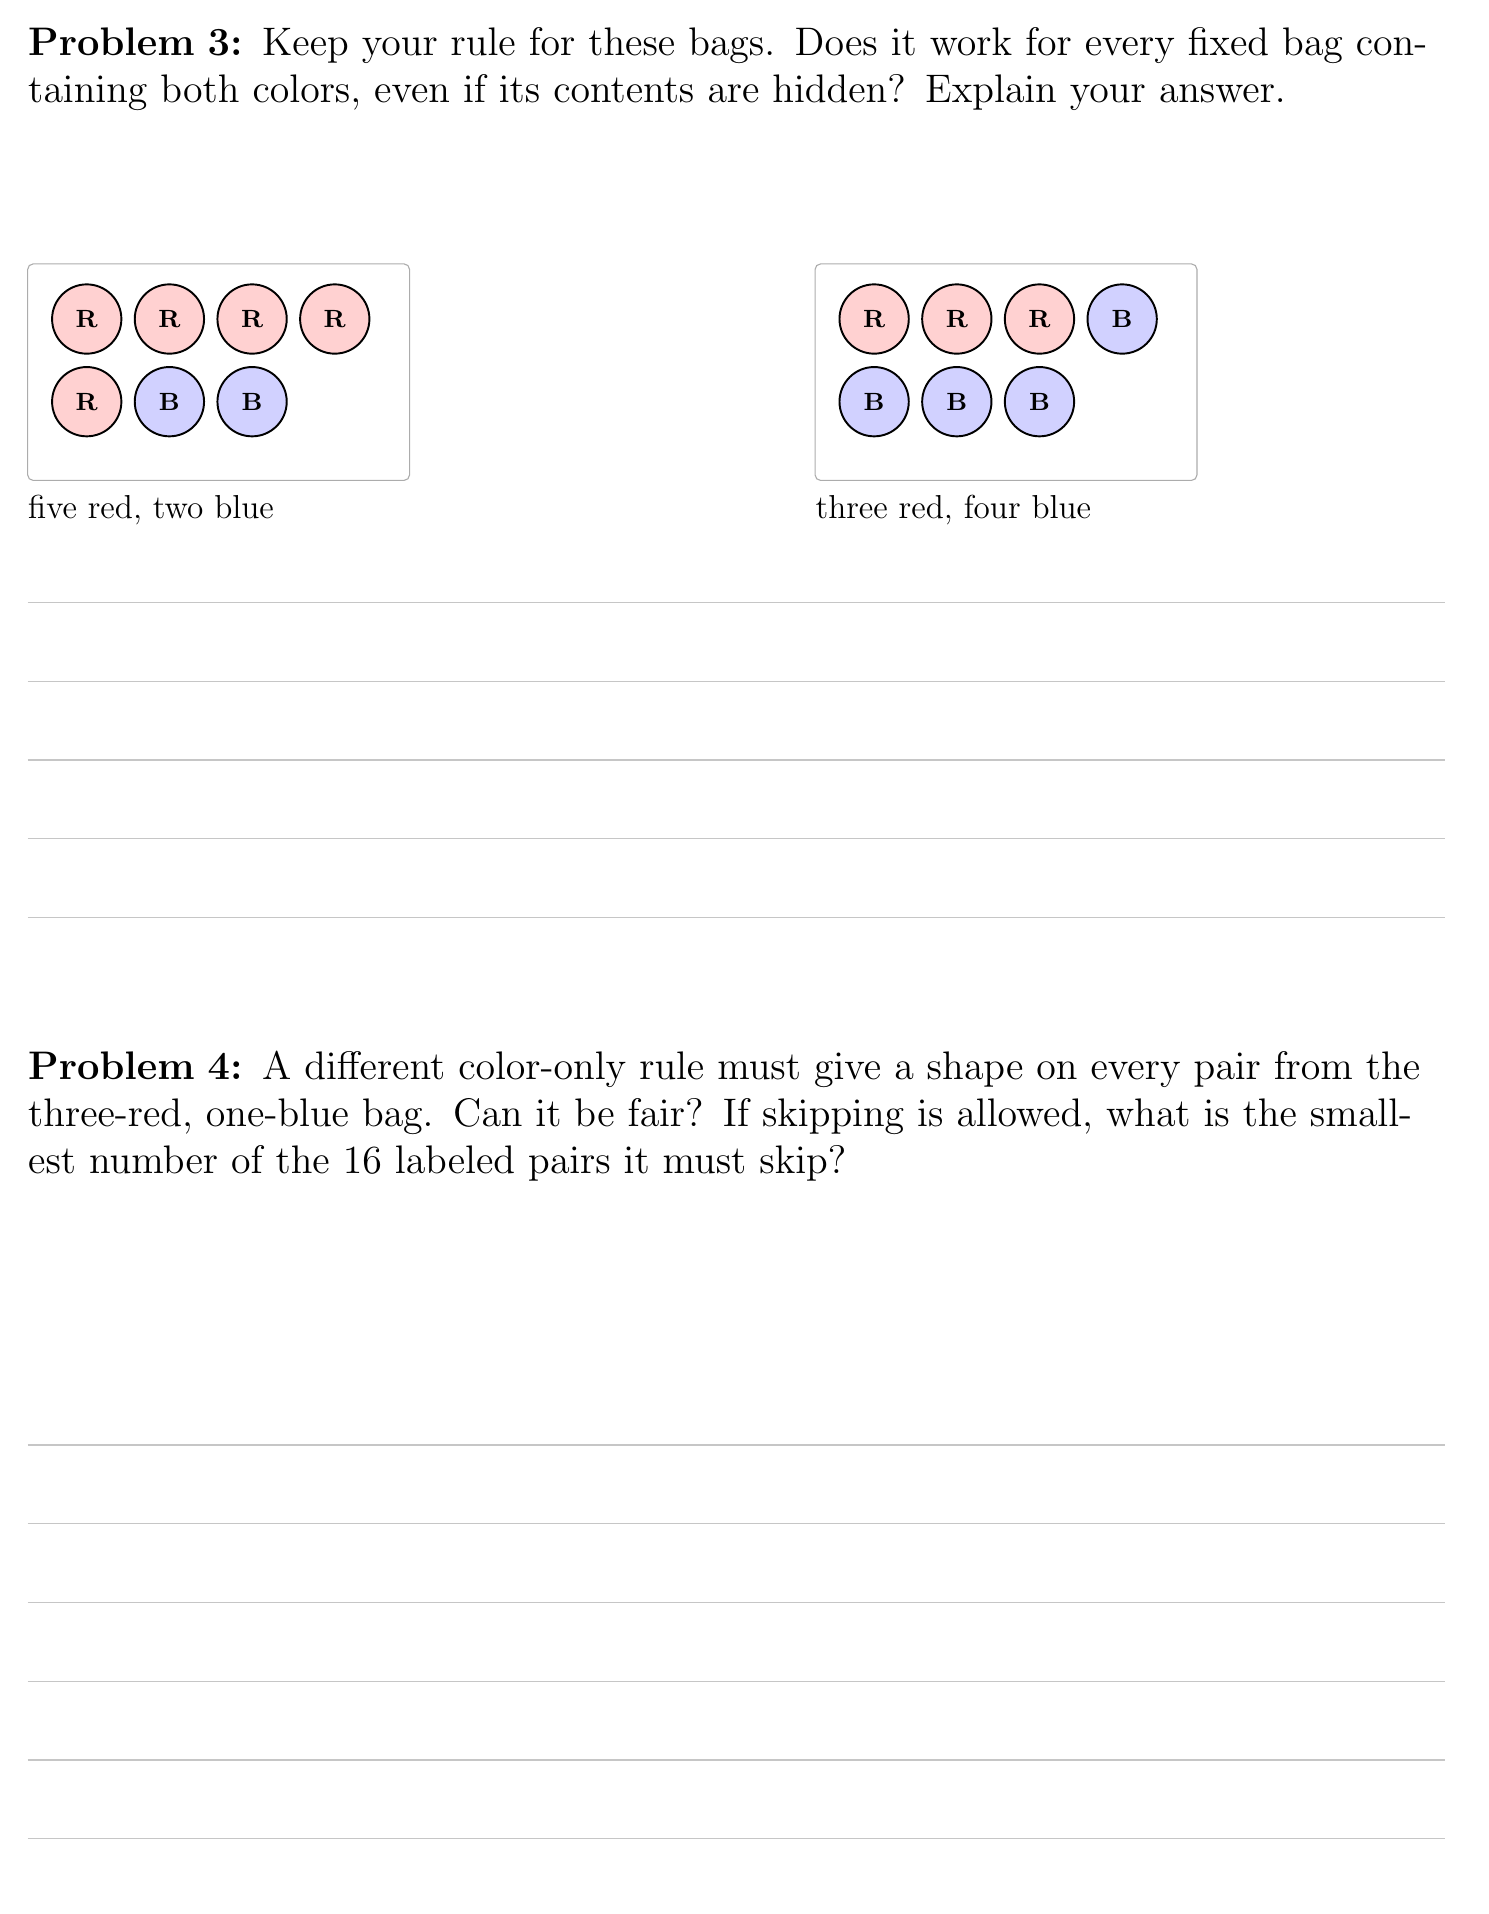
\begin{tikzpicture}[x=1cm,y=1cm]\path[use as bounding box] (0,0) rectangle (18.2,-23.6);
\node[anchor=north west,text width=18cm,inner sep=0pt,font=\fontsize{14}{17}\selectfont] at (0,0) {\textbf{Problem 3:} Keep your rule for these bags. Does it work for every fixed bag containing both colors, even if its contents are hidden? Explain your answer.};
\draw[gray!65,rounded corners=2pt] (0,-3) rectangle (4.8500000000000005,-5.75);
\draw[fill=red!18,line width=.7pt] (0.75,-3.7) circle (0.44);
\node[font=\bfseries\small] at (0.75,-3.7) {R};
\draw[fill=red!18,line width=.7pt] (1.8,-3.7) circle (0.44);
\node[font=\bfseries\small] at (1.8,-3.7) {R};
\draw[fill=red!18,line width=.7pt] (2.85,-3.7) circle (0.44);
\node[font=\bfseries\small] at (2.85,-3.7) {R};
\draw[fill=red!18,line width=.7pt] (3.9000000000000004,-3.7) circle (0.44);
\node[font=\bfseries\small] at (3.9000000000000004,-3.7) {R};
\draw[fill=red!18,line width=.7pt] (0.75,-4.75) circle (0.44);
\node[font=\bfseries\small] at (0.75,-4.75) {R};
\draw[fill=blue!18,line width=.7pt] (1.8,-4.75) circle (0.44);
\node[font=\bfseries\small] at (1.8,-4.75) {B};
\draw[fill=blue!18,line width=.7pt] (2.85,-4.75) circle (0.44);
\node[font=\bfseries\small] at (2.85,-4.75) {B};
\node[anchor=north west,text width=4.8500000000000005cm,inner sep=0pt,font=\fontsize{12}{15}\selectfont] at (0,-5.93) {five red, two blue};
\draw[gray!65,rounded corners=2pt] (10,-3) rectangle (14.850000000000001,-5.75);
\draw[fill=red!18,line width=.7pt] (10.75,-3.7) circle (0.44);
\node[font=\bfseries\small] at (10.75,-3.7) {R};
\draw[fill=red!18,line width=.7pt] (11.8,-3.7) circle (0.44);
\node[font=\bfseries\small] at (11.8,-3.7) {R};
\draw[fill=red!18,line width=.7pt] (12.85,-3.7) circle (0.44);
\node[font=\bfseries\small] at (12.85,-3.7) {R};
\draw[fill=blue!18,line width=.7pt] (13.9,-3.7) circle (0.44);
\node[font=\bfseries\small] at (13.9,-3.7) {B};
\draw[fill=blue!18,line width=.7pt] (10.75,-4.75) circle (0.44);
\node[font=\bfseries\small] at (10.75,-4.75) {B};
\draw[fill=blue!18,line width=.7pt] (11.8,-4.75) circle (0.44);
\node[font=\bfseries\small] at (11.8,-4.75) {B};
\draw[fill=blue!18,line width=.7pt] (12.85,-4.75) circle (0.44);
\node[font=\bfseries\small] at (12.85,-4.75) {B};
\node[anchor=north west,text width=4.8500000000000005cm,inner sep=0pt,font=\fontsize{12}{15}\selectfont] at (10,-5.93) {three red, four blue};
\draw[gray!45] (0,-7.3) -- (18,-7.3);
\draw[gray!45] (0,-8.3) -- (18,-8.3);
\draw[gray!45] (0,-9.3) -- (18,-9.3);
\draw[gray!45] (0,-10.3) -- (18,-10.3);
\draw[gray!45] (0,-11.3) -- (18,-11.3);
\node[anchor=north west,text width=18cm,inner sep=0pt,font=\fontsize{14}{17}\selectfont] at (0,-13) {\textbf{Problem 4:} A different color-only rule must give a shape on every pair from the three-red, one-blue bag. Can it be fair? If skipping is allowed, what is the smallest number of the 16 labeled pairs it must skip?};
\draw[gray!45] (0,-18) -- (18,-18);
\draw[gray!45] (0,-19) -- (18,-19);
\draw[gray!45] (0,-20) -- (18,-20);
\draw[gray!45] (0,-21) -- (18,-21);
\draw[gray!45] (0,-22) -- (18,-22);
\draw[gray!45] (0,-23) -- (18,-23);
\end{tikzpicture}
\newpage
\noindent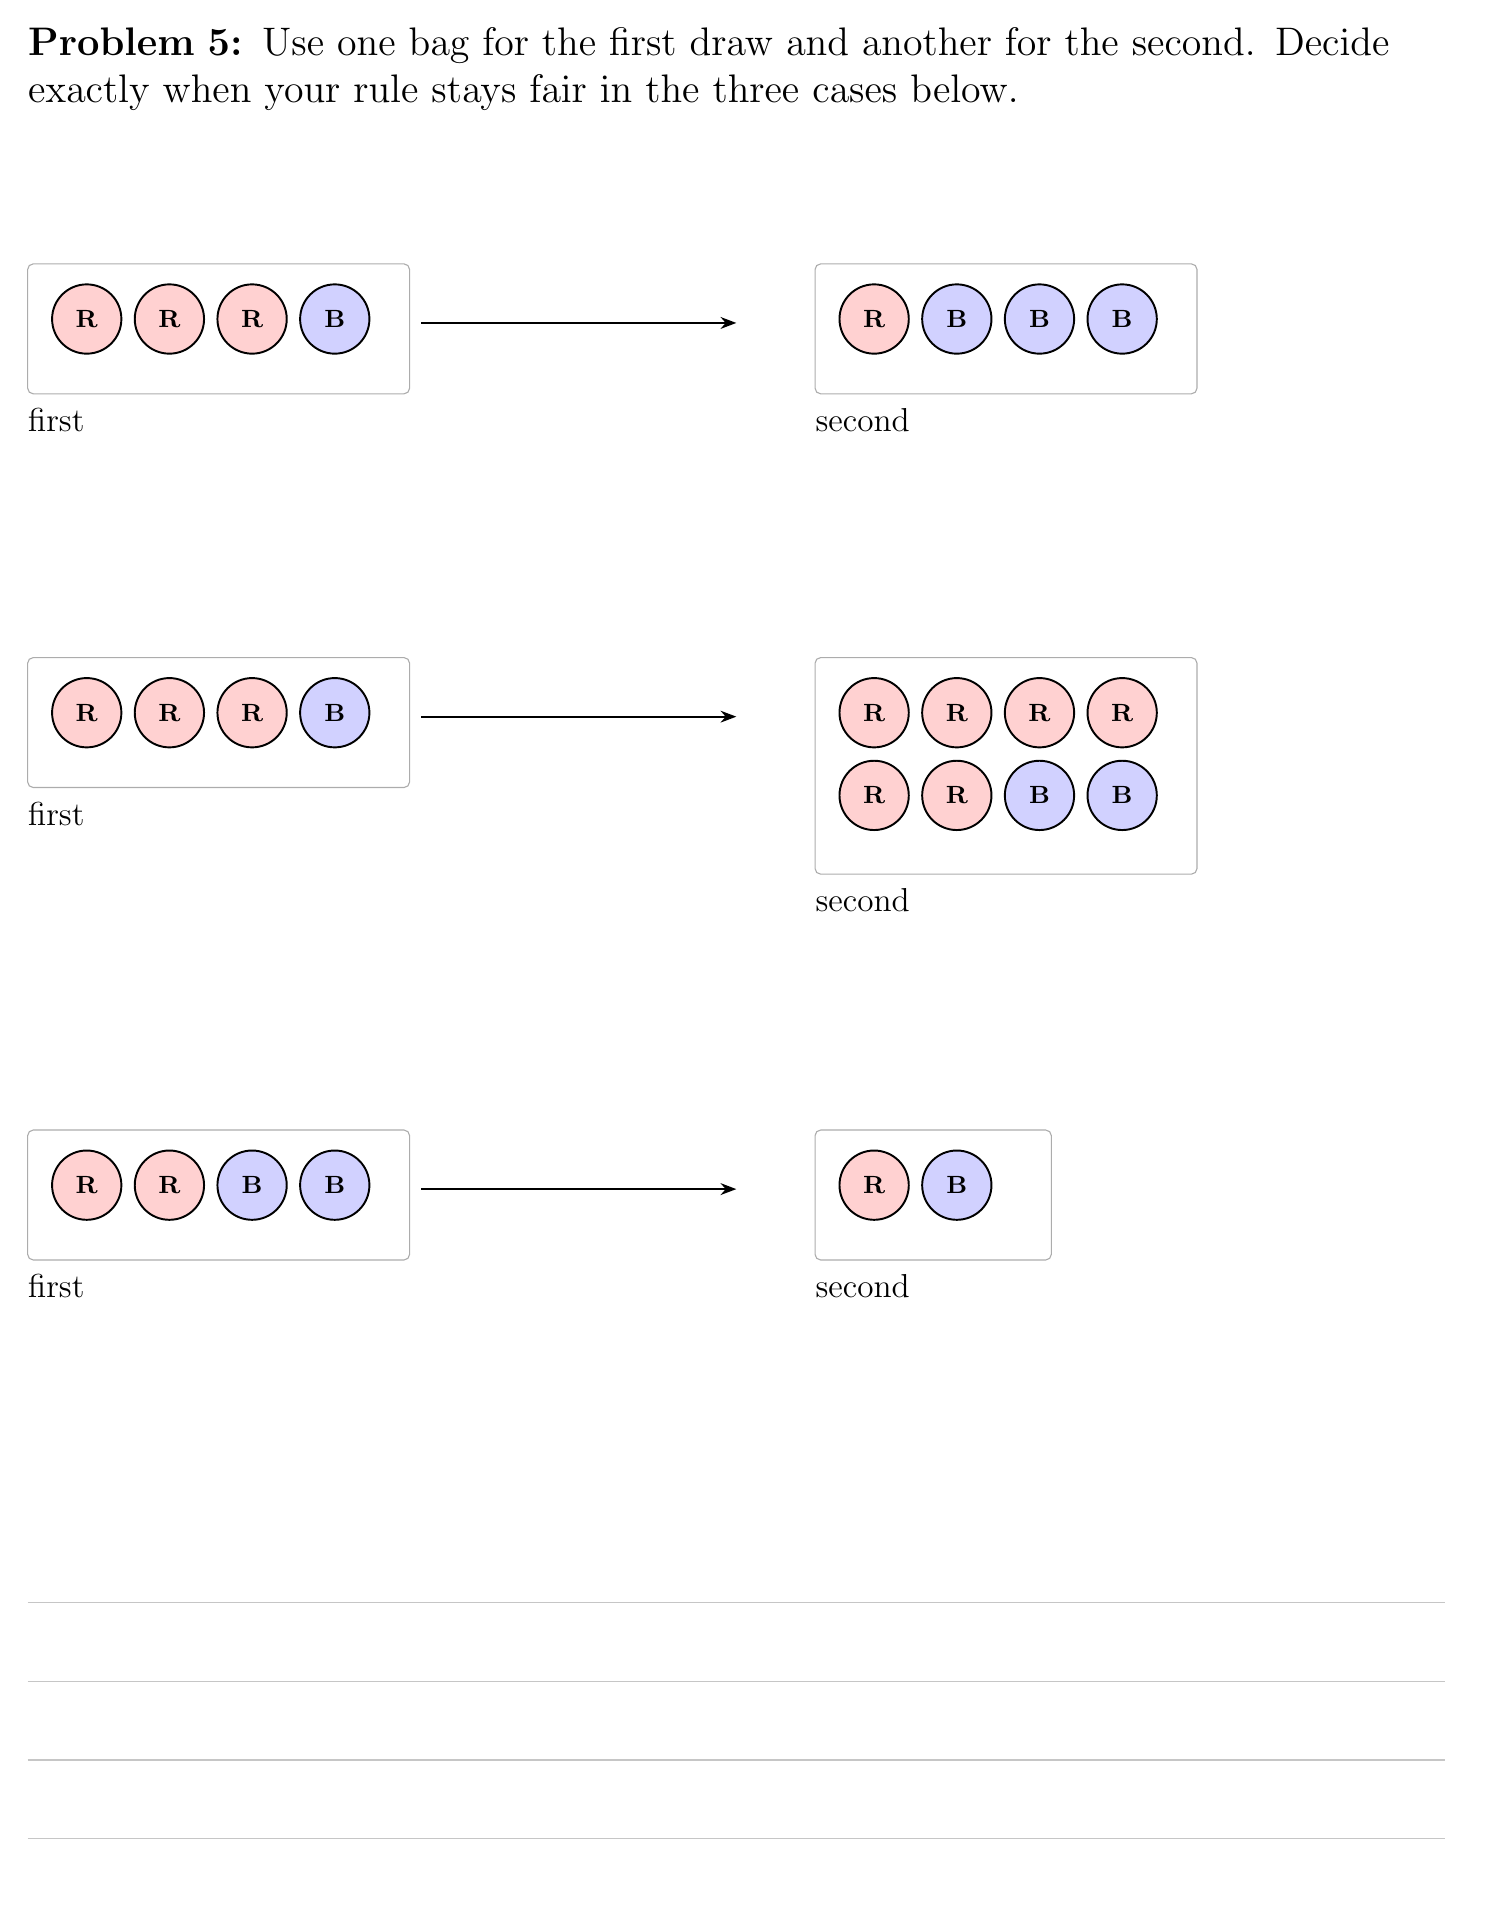
\begin{tikzpicture}[x=1cm,y=1cm]\path[use as bounding box] (0,0) rectangle (18.2,-23.6);
\node[anchor=north west,text width=18cm,inner sep=0pt,font=\fontsize{14}{17}\selectfont] at (0,0) {\textbf{Problem 5:} Use one bag for the first draw and another for the second. Decide exactly when your rule stays fair in the three cases below.};
\draw[gray!65,rounded corners=2pt] (0,-3) rectangle (4.8500000000000005,-4.65);
\draw[fill=red!18,line width=.7pt] (0.75,-3.7) circle (0.44);
\node[font=\bfseries\small] at (0.75,-3.7) {R};
\draw[fill=red!18,line width=.7pt] (1.8,-3.7) circle (0.44);
\node[font=\bfseries\small] at (1.8,-3.7) {R};
\draw[fill=red!18,line width=.7pt] (2.85,-3.7) circle (0.44);
\node[font=\bfseries\small] at (2.85,-3.7) {R};
\draw[fill=blue!18,line width=.7pt] (3.9000000000000004,-3.7) circle (0.44);
\node[font=\bfseries\small] at (3.9000000000000004,-3.7) {B};
\node[anchor=north west,text width=4.8500000000000005cm,inner sep=0pt,font=\fontsize{12}{15}\selectfont] at (0,-4.83) {first};
\draw[gray!65,rounded corners=2pt] (10,-3) rectangle (14.850000000000001,-4.65);
\draw[fill=red!18,line width=.7pt] (10.75,-3.7) circle (0.44);
\node[font=\bfseries\small] at (10.75,-3.7) {R};
\draw[fill=blue!18,line width=.7pt] (11.8,-3.7) circle (0.44);
\node[font=\bfseries\small] at (11.8,-3.7) {B};
\draw[fill=blue!18,line width=.7pt] (12.85,-3.7) circle (0.44);
\node[font=\bfseries\small] at (12.85,-3.7) {B};
\draw[fill=blue!18,line width=.7pt] (13.9,-3.7) circle (0.44);
\node[font=\bfseries\small] at (13.9,-3.7) {B};
\node[anchor=north west,text width=4.8500000000000005cm,inner sep=0pt,font=\fontsize{12}{15}\selectfont] at (10,-4.83) {second};
\draw[-{Stealth[length=2mm]},line width=.8pt] (5,-3.75) -- (9,-3.75) node[midway,above,font=\small] {};
\draw[gray!65,rounded corners=2pt] (0,-8) rectangle (4.8500000000000005,-9.65);
\draw[fill=red!18,line width=.7pt] (0.75,-8.7) circle (0.44);
\node[font=\bfseries\small] at (0.75,-8.7) {R};
\draw[fill=red!18,line width=.7pt] (1.8,-8.7) circle (0.44);
\node[font=\bfseries\small] at (1.8,-8.7) {R};
\draw[fill=red!18,line width=.7pt] (2.85,-8.7) circle (0.44);
\node[font=\bfseries\small] at (2.85,-8.7) {R};
\draw[fill=blue!18,line width=.7pt] (3.9000000000000004,-8.7) circle (0.44);
\node[font=\bfseries\small] at (3.9000000000000004,-8.7) {B};
\node[anchor=north west,text width=4.8500000000000005cm,inner sep=0pt,font=\fontsize{12}{15}\selectfont] at (0,-9.83) {first};
\draw[gray!65,rounded corners=2pt] (10,-8) rectangle (14.850000000000001,-10.75);
\draw[fill=red!18,line width=.7pt] (10.75,-8.7) circle (0.44);
\node[font=\bfseries\small] at (10.75,-8.7) {R};
\draw[fill=red!18,line width=.7pt] (11.8,-8.7) circle (0.44);
\node[font=\bfseries\small] at (11.8,-8.7) {R};
\draw[fill=red!18,line width=.7pt] (12.85,-8.7) circle (0.44);
\node[font=\bfseries\small] at (12.85,-8.7) {R};
\draw[fill=red!18,line width=.7pt] (13.9,-8.7) circle (0.44);
\node[font=\bfseries\small] at (13.9,-8.7) {R};
\draw[fill=red!18,line width=.7pt] (10.75,-9.75) circle (0.44);
\node[font=\bfseries\small] at (10.75,-9.75) {R};
\draw[fill=red!18,line width=.7pt] (11.8,-9.75) circle (0.44);
\node[font=\bfseries\small] at (11.8,-9.75) {R};
\draw[fill=blue!18,line width=.7pt] (12.85,-9.75) circle (0.44);
\node[font=\bfseries\small] at (12.85,-9.75) {B};
\draw[fill=blue!18,line width=.7pt] (13.9,-9.75) circle (0.44);
\node[font=\bfseries\small] at (13.9,-9.75) {B};
\node[anchor=north west,text width=4.8500000000000005cm,inner sep=0pt,font=\fontsize{12}{15}\selectfont] at (10,-10.93) {second};
\draw[-{Stealth[length=2mm]},line width=.8pt] (5,-8.75) -- (9,-8.75) node[midway,above,font=\small] {};
\draw[gray!65,rounded corners=2pt] (0,-14) rectangle (4.8500000000000005,-15.65);
\draw[fill=red!18,line width=.7pt] (0.75,-14.7) circle (0.44);
\node[font=\bfseries\small] at (0.75,-14.7) {R};
\draw[fill=red!18,line width=.7pt] (1.8,-14.7) circle (0.44);
\node[font=\bfseries\small] at (1.8,-14.7) {R};
\draw[fill=blue!18,line width=.7pt] (2.85,-14.7) circle (0.44);
\node[font=\bfseries\small] at (2.85,-14.7) {B};
\draw[fill=blue!18,line width=.7pt] (3.9000000000000004,-14.7) circle (0.44);
\node[font=\bfseries\small] at (3.9000000000000004,-14.7) {B};
\node[anchor=north west,text width=4.8500000000000005cm,inner sep=0pt,font=\fontsize{12}{15}\selectfont] at (0,-15.83) {first};
\draw[gray!65,rounded corners=2pt] (10,-14) rectangle (13,-15.65);
\draw[fill=red!18,line width=.7pt] (10.75,-14.7) circle (0.44);
\node[font=\bfseries\small] at (10.75,-14.7) {R};
\draw[fill=blue!18,line width=.7pt] (11.8,-14.7) circle (0.44);
\node[font=\bfseries\small] at (11.8,-14.7) {B};
\node[anchor=north west,text width=3cm,inner sep=0pt,font=\fontsize{12}{15}\selectfont] at (10,-15.83) {second};
\draw[-{Stealth[length=2mm]},line width=.8pt] (5,-14.75) -- (9,-14.75) node[midway,above,font=\small] {};
\draw[gray!45] (0,-20) -- (18,-20);
\draw[gray!45] (0,-21) -- (18,-21);
\draw[gray!45] (0,-22) -- (18,-22);
\draw[gray!45] (0,-23) -- (18,-23);
\end{tikzpicture}
\newpage
\noindent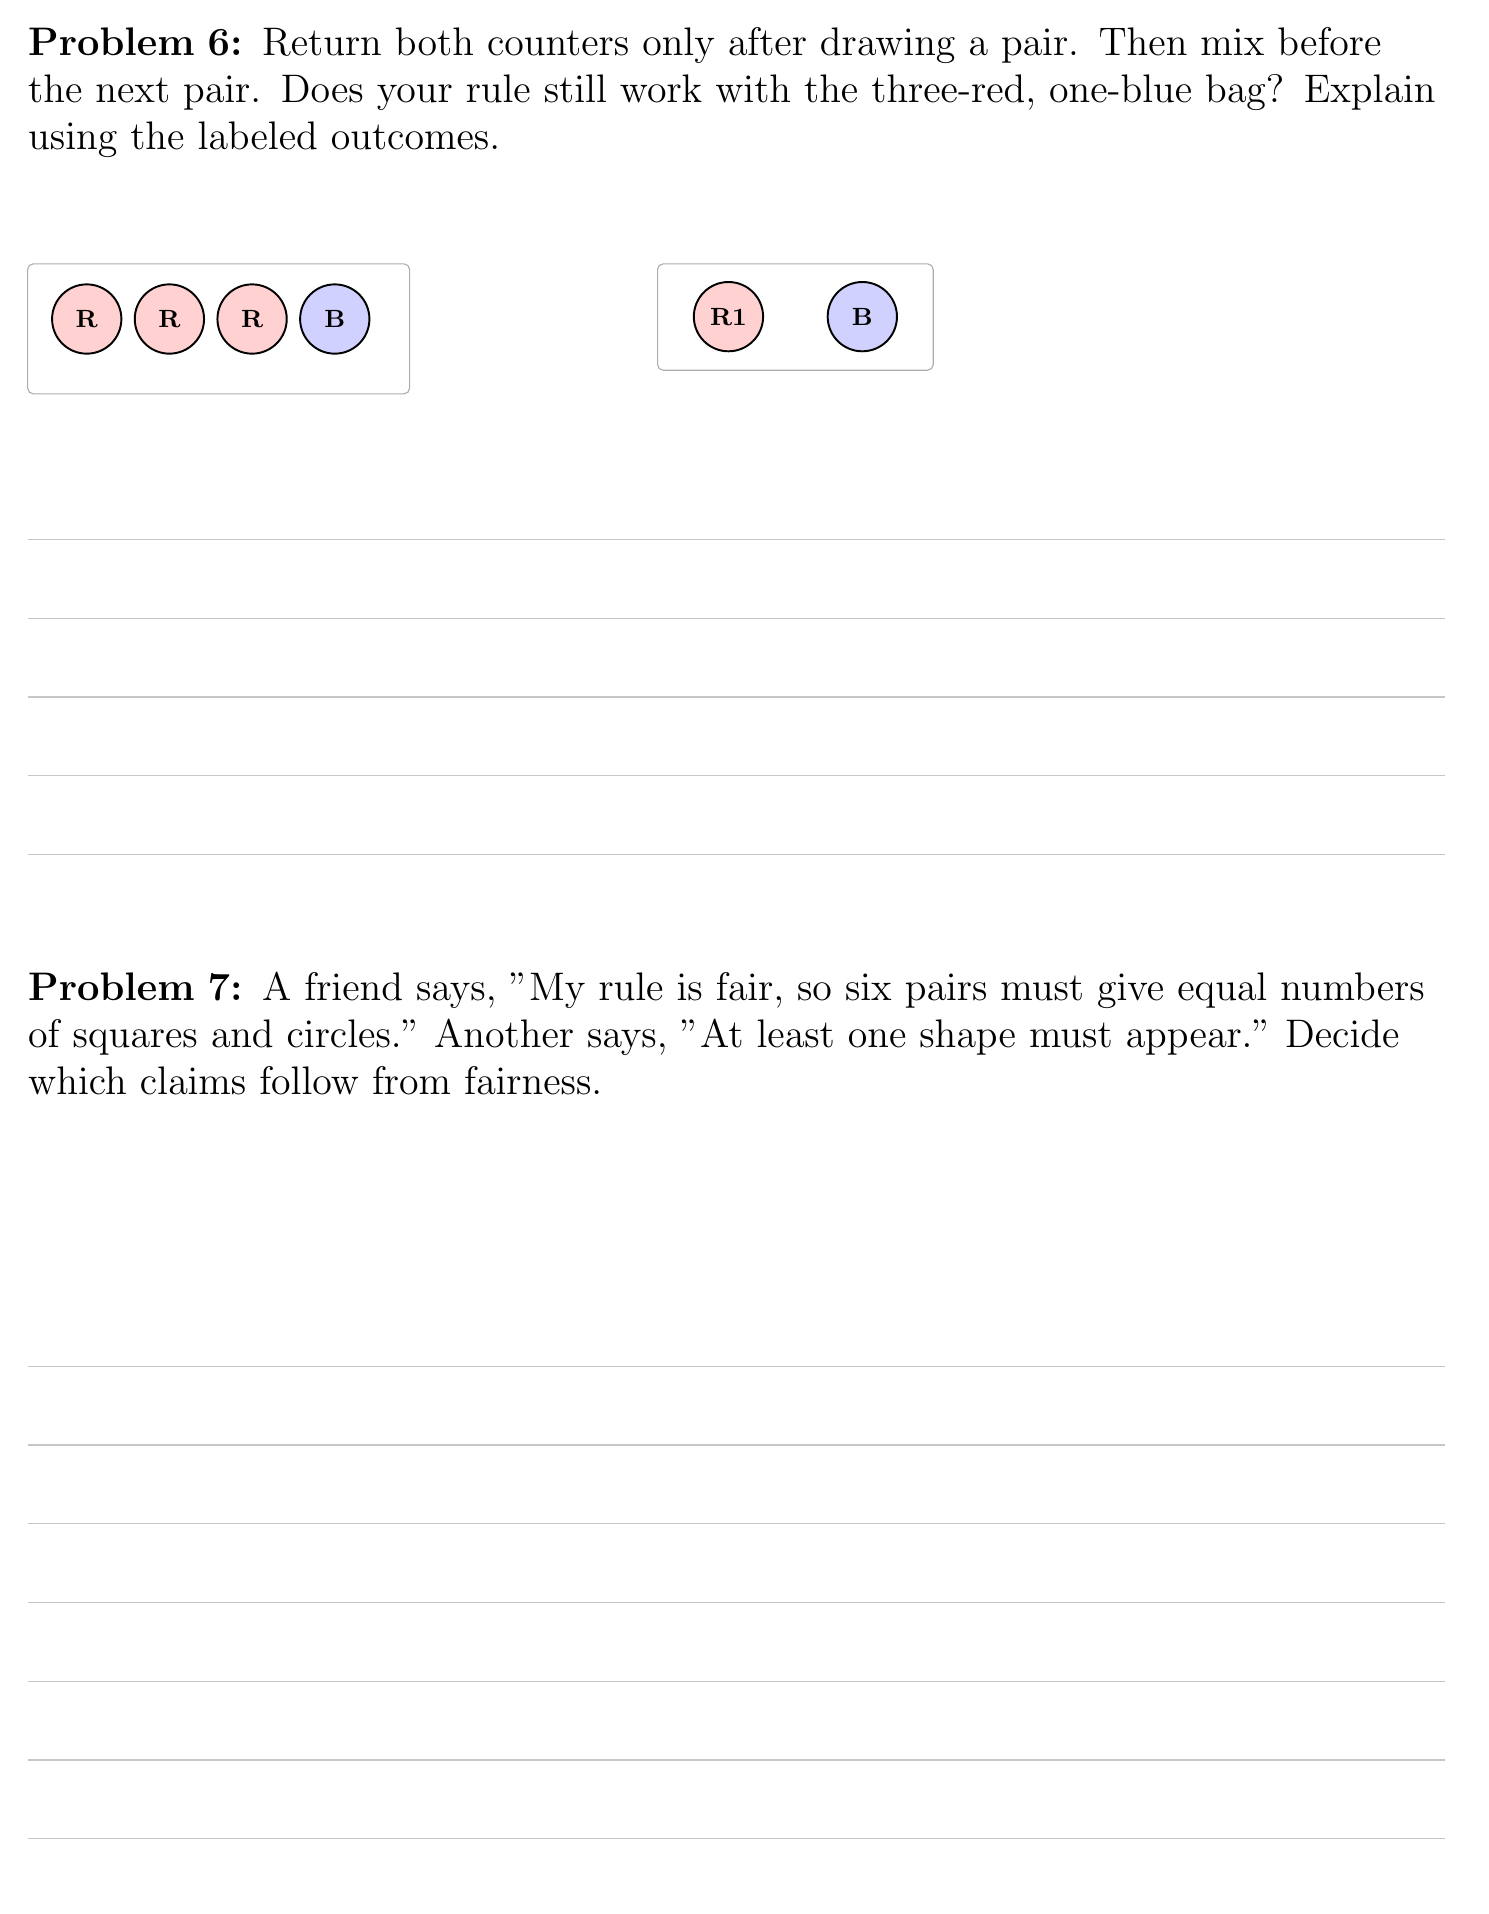
\begin{tikzpicture}[x=1cm,y=1cm]\path[use as bounding box] (0,0) rectangle (18.2,-23.6);
\node[anchor=north west,text width=18cm,inner sep=0pt,font=\fontsize{14}{17}\selectfont] at (0,0) {\textbf{Problem 6:} Return both counters only after drawing a pair. Then mix before the next pair. Does your rule still work with the three-red, one-blue bag? Explain using the labeled outcomes.};
\draw[gray!65,rounded corners=2pt] (0,-3) rectangle (4.8500000000000005,-4.65);
\draw[fill=red!18,line width=.7pt] (0.75,-3.7) circle (0.44);
\node[font=\bfseries\small] at (0.75,-3.7) {R};
\draw[fill=red!18,line width=.7pt] (1.8,-3.7) circle (0.44);
\node[font=\bfseries\small] at (1.8,-3.7) {R};
\draw[fill=red!18,line width=.7pt] (2.85,-3.7) circle (0.44);
\node[font=\bfseries\small] at (2.85,-3.7) {R};
\draw[fill=blue!18,line width=.7pt] (3.9000000000000004,-3.7) circle (0.44);
\node[font=\bfseries\small] at (3.9000000000000004,-3.7) {B};
\draw[gray!65,rounded corners=2pt] (8,-3) rectangle (11.5,-4.35);
\draw[fill=red!18,line width=.7pt] (8.9,-3.67) circle (0.44);
\node[font=\bfseries\small] at (8.9,-3.67) {R1};
\draw[fill=blue!18,line width=.7pt] (10.6,-3.67) circle (0.44);
\node[font=\bfseries\small] at (10.6,-3.67) {B};
\draw[gray!45] (0,-6.5) -- (18,-6.5);
\draw[gray!45] (0,-7.5) -- (18,-7.5);
\draw[gray!45] (0,-8.5) -- (18,-8.5);
\draw[gray!45] (0,-9.5) -- (18,-9.5);
\draw[gray!45] (0,-10.5) -- (18,-10.5);
\node[anchor=north west,text width=18cm,inner sep=0pt,font=\fontsize{14}{17}\selectfont] at (0,-12) {\textbf{Problem 7:} A friend says, "My rule is fair, so six pairs must give equal numbers of squares and circles." Another says, "At least one shape must appear." Decide which claims follow from fairness.};
\draw[gray!45] (0,-17) -- (18,-17);
\draw[gray!45] (0,-18) -- (18,-18);
\draw[gray!45] (0,-19) -- (18,-19);
\draw[gray!45] (0,-20) -- (18,-20);
\draw[gray!45] (0,-21) -- (18,-21);
\draw[gray!45] (0,-22) -- (18,-22);
\draw[gray!45] (0,-23) -- (18,-23);
\end{tikzpicture}
\end{document}
